\documentclass[12pt, twoside]{article}
\usepackage[letterpaper, margin=1in, headsep=0.5in]{geometry}
\usepackage[english]{babel}
\usepackage[utf8]{inputenc}
\usepackage{amsmath}
\usepackage{amsfonts}
\usepackage{amssymb}
\usepackage{tikz}
\usetikzlibrary{quotes, angles}

\usepackage{pgfplots}
\pgfplotsset{width=9cm,compat=1.9}
\usepgfplotslibrary{statistics}
\usepackage{pgfplotstable}

\usepackage{venndiagram}

\usepackage{graphicx}
\usepackage{enumitem}
\usepackage{multicol}
\usepackage{hyperref}

\newif\ifmeta
\metatrue %print standards and topics tags

\title{IB Mathematics}
\author{Chris Huson}
\date{November 2021}

\usepackage{fancyhdr}
\pagestyle{fancy}
\fancyhf{}
\renewcommand{\headrulewidth}{0pt} % disable the underline of the header
\raggedbottom

\fancyhead[LE]{\thepage}
\fancyhead[RO]{\thepage \\ Name: \hspace{4cm} \,\\}
\fancyhead[LO]{BECA / IB Math 02-Descriptive Statistics\\* 14 December 2021}

\begin{document}
\subsubsection*{2.5 Classwork: Linear regression}
\begin{enumerate}
\item The box-and-whisker plot represents the examination scores of a group of students. The range of the scores is 42 marks, and the interquartile range is 18 marks.
  \begin{center}
  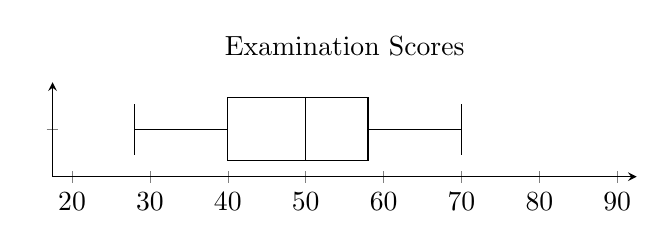
\begin{tikzpicture}[scale=1.0]
    \begin{axis}[
        title={Examination Scores},
        axis lines=left,
        xmin=30, xmax=80,
        y=1cm,
        ytick={1},
        yticklabels={},
      enlargelimits=0.25,
        ]
        %\addplot+ [boxplot]
        %table {3-11_IB-exam.txt};
       \addplot [boxplot prepared={draw position=1,
            lower whisker=28, lower quartile=40,
            median=50,
            upper quartile=58, upper whisker=70,
            %average=28,
            },
        ] coordinates {};
    \end{axis}
    \end{tikzpicture}
  \end{center}
  \begin{enumerate}
    \item Find the value of
    \begin{enumerate}
      \item the minimum score; \vspace{1cm}
      \item the third quartile. 
    \end{enumerate} \vspace{0.5cm}
    \item What percentage of the students scored below 40?
  \end{enumerate}

\item The flash rate of fireflies depends on various factors, including temperature. Firefly field data (simulated) where $T$ is the temperature and $f(T)$ is the number of seconds between flashes is shown below.\\[0.25cm]
Plot the data in the table on the grid below (one point is plotted for you) and draw a line of best fit.
  \begin{center}
    \begin{tabular}{|c|r|r|r|r|r|}
    \hline
    $T$ & 54 & 60 & 64 & 70 & 75 \\ [3pt]
    \hline
    $f(T)$ & 5 & 8 & 10 & 11 & 13  \\  [3pt]
    \hline
    \end{tabular}
  \end{center}
  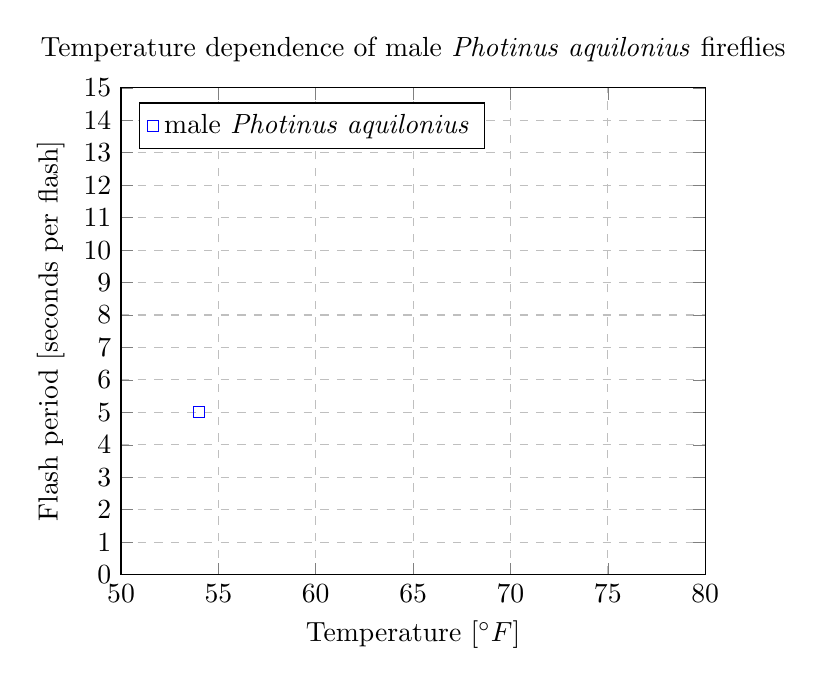
\begin{tikzpicture}[scale=1.0]
  \begin{axis}[
      title={Temperature dependence of male \emph{Photinus aquilonius} fireflies},
      xlabel={Temperature [$^{\circ}F$]},
      ylabel={Flash period [seconds per flash]},
      xmin=50, xmax=80,
      ymin=0, ymax=15,
      xtick={50,55,60,65,70,75,80},
      ytick={0,1,2,3,4,5,6,7,8,9,10,11,12,13,14,15},
      legend pos=north west,
      xmajorgrids=true,
      ymajorgrids=true,
      grid style=dashed,
  ]
  \addplot[only marks,
      color=blue,
      mark=square,
      ]
      coordinates {
      (54,5)%(60,8)(64,10)(70,11)(75,13)
      };
      \legend{male \emph{Photinus aquilonius}}
  \end{axis}
  \end{tikzpicture}

\newpage
\item The histogram below shows the heart rate $x$ in beats per minute for 65 athletes after a fitness exercise.
  \begin{center}
    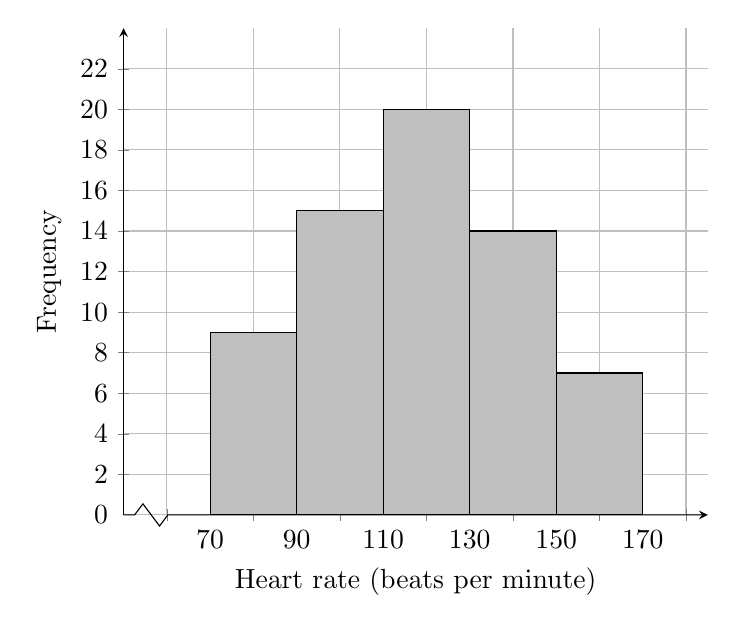
\begin{tikzpicture}
    \begin{axis}[
      xlabel=Heart rate (beats per minute),
      ylabel=Frequency,
      ybar interval=1,
      xmin=60, xmax=195,
      ymin=0, ymax=24,
      xtick={70,90,110,130,150,170,190},
      ytick={0,2,4,6,8,10,12,14,16,18,20,22},
      axis lines = left,
      ymajorgrids=true,
      axis x discontinuity=crunch,
    ]
    \addplot+ [color=black, fill=lightgray]
      coordinates {(80,9) (100,15)
        (120,20) (140,14) 
        (160,7) 
        (180,3)}; %Last pair does not show
    \end{axis}
    \end{tikzpicture}
  \end{center}
  The following is the frequency table for the distribution of $x$. \\[0.25cm]
    \begin{tabular}{|l|c|c|c|c|c|}
      \hline
      HR ($x$) & $70 \leq x < 90$ & $90 \leq x < 110$ & $110 \leq x < 130$ & $130 \leq x < 150$ & $150 \leq x < 170$ \\ 
      \hline 
      Freq & 9 & $p$ & 20 & 14 & 7  \\ 
      \hline 
      \end{tabular}
  \begin{enumerate}
    \item Write down the value of $p$. \hfill [1 mark] \vspace{1cm}
    \item Write down the modal class. \hfill [2 marks] \vspace{1cm}
    \item What percentage of the athletes have a heart rate of 130 beats per minute or greater? \hfill [2 marks] \vspace{1cm}
    \item Consider the class interval $70 \leq x < 90$.
    \begin{enumerate}
      \item Write down the interval width. \hfill [1 mark] \vspace{1cm}
      \item Write down the mid-interval value. \hfill [1 mark] 
    \end{enumerate}
    \item Hence find an estimate for the
    \begin{enumerate}
      \item mean; \hfill [2 marks] \vspace{1cm}
      \item standard deviation. \hfill [2 marks] 
    \end{enumerate}
  \end{enumerate}

\newpage
\item Dr. Huson buys a new plant and measures how tall it is after a number of weeks. Some of his measurements are shown below. Plot the points in the grid below.
  \renewcommand{\arraystretch}{1.6}
    \begin{center}
      \begin{tabular}{|l|r|r|r|r|}
      \hline
      Weeks & 2 & 5 & 7 & 10\\
      \hline
      Height (cm) & 5 & 6 & 8 & 9 \\
      \hline
      \end{tabular}
    \end{center}

\begin{center} %4 quadrant regents grid w T-Chart
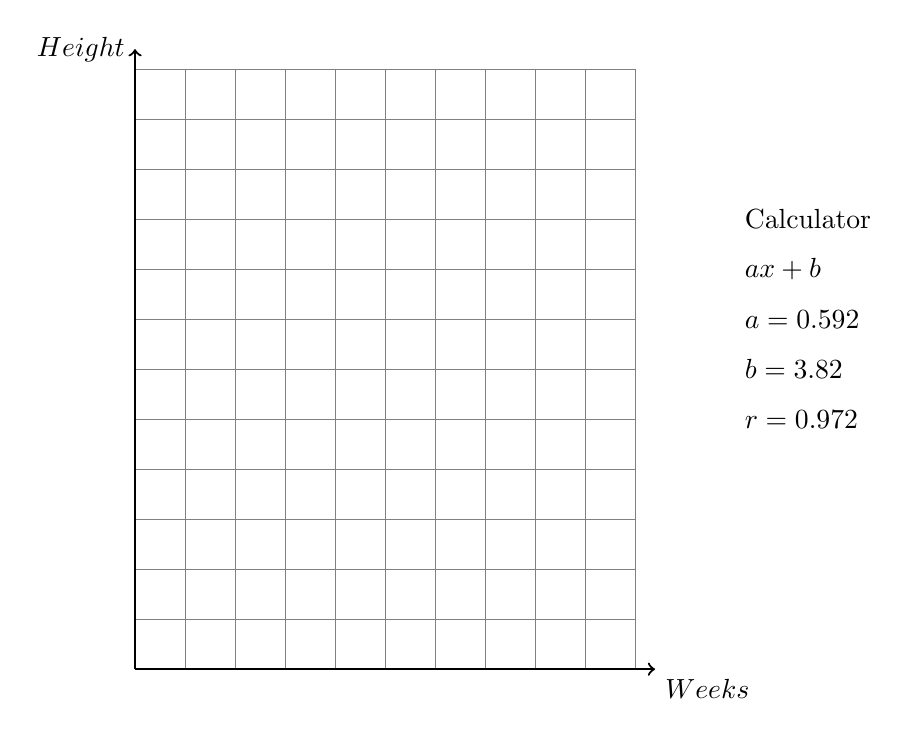
\begin{tikzpicture}[scale=.635]
  \draw [help lines] (0,0) grid (10,12);
  \draw [thick, ->] (0,0) -- (10.4,0) node [below right] {$Weeks$};
  \draw [thick, ->] (0,0)--(0,12.4) node [left] {$Height$};
  \node at (12,9)[right]{Calculator};
  \node at (12,8)[right]{$ax+b$};
  \node at (12,7)[right]{$a=0.592$};
  \node at (12,6)[right]{$b=3.82$};
  \node at (12,5)[right]{$r=0.972$};
\end{tikzpicture}
\end{center}
State, to the \emph{nearest tenth}, the linear regression equation that approximates the height, $y$, of the plants after $x$ weeks.\\[2cm]
Explain what the $y$-intercept means in the context of the problem. \\[3cm]
Explain what the slope means in the context of the problem.

\newpage
\item An environmental group records the numbers of coyotes and foxes in a wildlife reserve after $t$ years, starting on 1 January 1995.\\[0.25cm]
  Let $c$ be the number of coyotes in the reserve after $t$ years. The following table shows the number of coyotes after $t$ years.
    \begin{center}
      \begin{tabular}{|l|c|c|c|c|c|}
        \hline
        number of years ($t$) & 0 & 2 & 10 & 15 & 19 \\ 
        \hline 
        number of coyotes ($c$) & 115 & 197 & 265 & 320 & 406  \\ 
        \hline 
        \end{tabular}
      \end{center}
    The relationship between the variables can be modelled by the regression equation $c=at+b$.
    \begin{enumerate}
      \item Find the value of $a$ and $b$. \hfill [3 marks] \vspace{3cm}
      \item Find Pearson's correlation coefficient $r$ and characterize its value. \hfill [2 marks] \vspace{3cm}
      \item Use the regression equation to estimate the number of coyotes in the reserve when $t=7$. \hfill [3 marks]
    \end{enumerate}

\newpage
\item There are 250 high school students at BECA ranging in age from 13 to 18 years old. The following table shows the frequencies of each age.
  \begin{center}
  \begin{tabular}{|l|r|r|r|r|r|r|}
    \hline
    Age (years) & 13 & 14 & 15 & 16 & 17 & 18\\ 
    \hline 
    Frequency & 27 & 53 & 60 & 55 & 43 & 12\\ 
    \hline 
    \end{tabular}
  \end{center}
  \begin{enumerate}
    %\item Calculate the value of $k$. \hfill [1 mark] \vspace{1.5cm}
    \item Write down the mode. \hfill [1 mark] \vspace{1.5cm}
    \item Find the value of the range. \hfill [1 marks] \vspace{1.5cm}
    \item Find the median. \hfill [1 marks] \vspace{1.5cm}
    \item Find the mean. \hfill [2 marks] \vspace{1.5cm}
    \item Find the standard deviation. \hfill [2 marks] \vspace{1.5cm}
    \item Four years later the same 250 people have moved on to college and career. Find the new values of the 
    \begin{enumerate}
      \item mean; \hfill [1 marks] \vspace{1.5cm}
      \item standard deviation. \hfill [1 marks]
    \end{enumerate}
  \end{enumerate}

\end{enumerate}
\end{document}